%----------------------------------------------------------------------------------------
%   PACKAGES AND DOCUMENT CONFIGURATIONS
%----------------------------------------------------------------------------------------

\documentclass[12pt]{article}
\usepackage[english]{babel}
\usepackage[utf8]{inputenc}
\usepackage{float}

\usepackage{graphicx,epstopdf}   %for embedding images and for conveting eps to pdf
\usepackage{subfig}              %for sub images
\usepackage[margin=1in,includefoot]{geometry}	%changes the margins of report to 1 in
\usepackage{lscape}

\usepackage{rotating}   %used for rotating figures
\usepackage[automake,nonumberlist]{glossaries}    %To use glossary
\usepackage{varwidth}
\usepackage{multicol}   %for making columns
\usepackage{amsmath}
\usepackage{appendix}
\usepackage{pdfpages}
\usepackage{empheq}

\usepackage[framed, numbered]{matlab-prettifier}    %to import matlab code

%----------------------------------------------------------------------------------------
%   Acronym/Glossary
%----------------------------------------------------------------------------------------
\makeglossaries
\loadglsentries{glossary}

%----------------------------------------------------------------------------------------
%   Document Start
%----------------------------------------------------------------------------------------

\begin{document}

\begin{titlepage}

\newcommand{\HRule}{\rule{\linewidth}{0.5mm}} % Defines a new command for the horizontal lines, change thickness here

\center % Center everything on the page
 
%----------------------------------------------------------------------------------------
%   HEADING SECTIONS
%----------------------------------------------------------------------------------------

\textsc{\LARGE MSE 480 Manufacturing Systems}\\[1.5cm] % Org Name
\textsc{\Large }\\[0.5cm] % course name
\textsc{\large }\\[0.5cm] % course title

%----------------------------------------------------------------------------------------
%   TITLE SECTION
%----------------------------------------------------------------------------------------

\HRule \\[0.4cm]
{ \huge \bfseries Lab 1:Machining}\\[0.4cm] % Title of report
\HRule \\[1.5cm]
 
%----------------------------------------------------------------------------------------
%   AUTHOR SECTION
%----------------------------------------------------------------------------------------

\begin{minipage}{0.4\textwidth}
    \begin{flushleft} \large
        \emph{Authors:}\\
        Parshant \textsc{Bombhi}\\
        Klark \textsc{Li}
    \end{flushleft}
\end{minipage}
\hfill
\begin{minipage}{0.4\textwidth}
    \begin{flushright} \large
        \emph{Student ID:} \\
        301255126\\
        301276715
    \end{flushright}
\end{minipage}
\vspace{10mm}
%----------------------------------------------------------------------------------------
%   DATE SECTION
%----------------------------------------------------------------------------------------

{\large February 8, 2019}\\[2cm] % Date, change the \today to a set date if you want to be precise

%----------------------------------------------------------------------------------------
%   LOGO SECTION
%----------------------------------------------------------------------------------------


\includegraphics[scale=2.0]{MSE-Logo.jpg}\\[1cm] %logo
%----------------------------------------------------------------------------------------

\vfill % Fill the rest of the page with whitespace

\end{titlepage}

%----------------------------------------------------------------------------------------
%   Table of Contents/Table of Figures
%----------------------------------------------------------------------------------------
\pagenumbering{roman} %sets numbering of page to roman
\tableofcontents	%makes table of contents
\addcontentsline{toc}{section}{\numberline{}Table Of Contents}	%adds TOC to TOC

\listoffigures
\addcontentsline{toc}{section}{\numberline{}List of Figures}	%adds list of figures to table of contents

 \listoftables
 \addcontentsline{toc}{section}{\numberline{}List of Tables}

\lstlistoflistings
\addcontentsline{toc}{section}{\numberline{}Listings}

% \printglossary
% \addcontentsline{toc}{section}{\numberline{}Glossary}	%adds glossary to table of contents
\pagebreak
%----------------------------------------------------------------------------------------
%   Main Body
%----------------------------------------------------------------------------------------
\setcounter{page}{1}	%resets the page numbering
\pagenumbering{arabic}	%sets numbering of page to arabic
\setlength{\parskip}{1em}

\section{Introduction}
In this lab we were to observe several full-immersion passes on the Haas Mini Mill and record the spindle load percentage. Using the spindle load percentage and our knowledge of metal cutting we were to determine the cutting force constant ($K_1$) and the edge force constant ($K_2$).

\section{Recorded Data}
While observing the cuts we recorded the percent spindle load the mill was experiencing. The data is listed below in table \ref{tab:percentload}

% Table generated by Excel2LaTeX from sheet 'Sheet1'
\begin{table}[htbp]
  \centering
  \caption{Recorded Percent Load for Cuts}
    \begin{tabular}{|l|rrrr|}
    \hline
          & \multicolumn{1}{l}{Cut \#1} & \multicolumn{1}{l}{Cut \#2} & \multicolumn{1}{l}{Cut \#3 } & \multicolumn{1}{l|}{Cut \#4} \\
    \hline
    Width of Cut, $2R$ (in) & 3/4   & 3/4   & 3/4   & 3/4 \\
    Depth of Cut, $a$ (in) & 0.1   & 0.1   & 0.15  & 0.15 \\
    Spindle Speed (rpm) & 2200  & 2200  & 2200  & 2200 \\
    Feed Rate, $S_t$ (in/tooth) & 0.034 & 0.0057 & 0.034 & 0.0057 \\
    \textbf{Spindle Load (\%)} & \textbf{25} & \textbf{31} & \textbf{33} & \textbf{42} \\
    \hline
    \end{tabular}%
  \label{tab:percentload}%
\end{table}%

We can also determine the max torque by looking in the lab manual for the torque vs spindle speed graph.
\begin{figure}[h!]
    \centering
    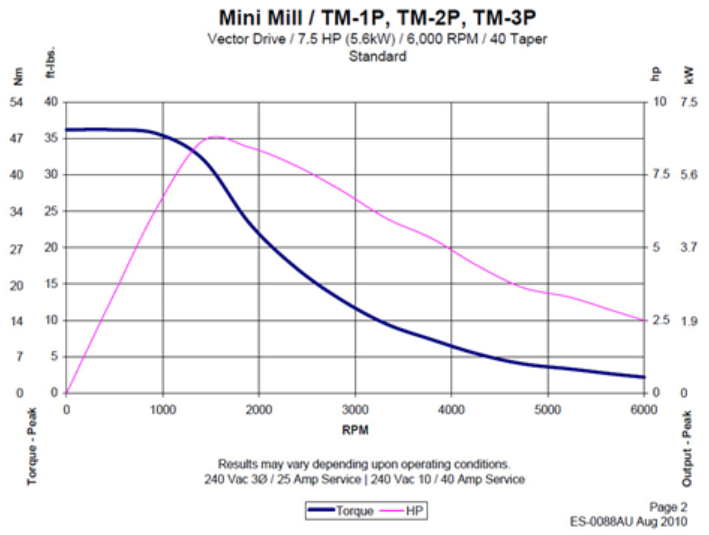
\includegraphics[width=0.5\textwidth]{rpm_vs_torque.png}
    \caption{Haas Mini Mill Spindle Torque vs RPM}
    \label{fig:rpmvstc}
\end{figure}

Using the graph in figure \ref{fig:rpmvstc} we can determine the cutting torque ($T_c$). It is important to note that the graph shows the resultant torque as 200\% of actual. At the 2,200 rpm that the mill was running at we have about 19 ft-lbs of torque. To make calculations a bit easier, this was changed to in-lbs by multiplying with 12. The cutting torques for each run are shown below in table \ref{tab:torques}

% Table generated by Excel2LaTeX from sheet 'Sheet1'
\begin{table}[htbp]
  \centering
  \caption{Cutting Torque}
    \begin{tabular}{|l|rrrr|}
    \hline
          & \multicolumn{1}{l}{Cut \#1} & \multicolumn{1}{l}{Cut \#2} & \multicolumn{1}{l}{Cut \#3 } & \multicolumn{1}{l|}{Cut \#4} \\
    \hline
    Torque (in-lbs) & 28.50 & 35.34 & 37.62 & 47.88 \\
    \hline
    \end{tabular}%
  \label{tab:torques}%
\end{table}%
\section{Theory}
The formula for the torque given is:
\begin{equation}
\label{eq:basicTc}
    T_c=RK_1aS_t\Big[sin\phi + \frac{h^*}{h_{eq}}\Big]
\end{equation}
From lecture notes on the turning process we know the formula for the power consuming force ($F_v$). We can use this formula to solve for the critical chip thickness ($h^*$).
\begin{align}
    F_v=K_1(L_eh_{eq}) + K_2L_2 &= K_1L_eh_{eq}\Big(1+\frac{h^*}{h_{eq}}\Big)\\
    K_1L_eh_{eq}+K_2L_e&=K_1L_eh_{eq}+K_1L_eh_{eq}\frac{h^*}{h_{eq}}\nonumber\\
    K_2&=K_1h^*\nonumber\\
    h^*&=\frac{K_2}{K_1}\label{eq:hstar}
\end{align}
From the notes we have the equation for the equivalent chip thickness ($h_{eq}$)
\begin{equation}
\label{eq:heq}
    h_{eq}=\frac{S_ta}{L_e}
\end{equation}
Substituting equations \ref{eq:hstar} and \ref{eq:heq} into equation \ref{eq:basicTc} we get:
\begin{equation}
    T_c=RK_1aS_tsin(\phi) + RK_2L_e
\end{equation}
Since we know the milling process is cyclical, the torque is a function of the cutter rotation angle ($\phi$). Thus to find the average torque we need to integrate the function with respect to $\phi$.
\begin{equation}
    \label{eq:Tc_given}
    T_c(\phi)=2\Big[\frac{RK_1aS_t\int_{0}^{\pi}sin(\phi) d\phi}{2\pi}+\frac{RK_2\int_{0}^{\pi}L_e(\phi) d\phi}{2\pi}\Big]
\end{equation}
If we assume $L_e$ to be constant we can solve the definite integrals and get:
\begin{equation}
    T_c=\frac{2RK_1aS_t}{\pi} + RK_2L_e
    \end{equation}

\section{Calculations/Results}
From the data sheet of the insert we can find the effective cutting edge ($L_e$) using the wiper edge length ($B_s$), corner radius ($R_e$) and depth of cut ($a$) . Note that in figure \ref{fig:insertfig} $L_e$ is show as the edge length of this insert. In our case this is not correct as our cut is in full-immersion and the depth of cut is less then the cutter height.

\begin{figure}[h!]
    \centering
    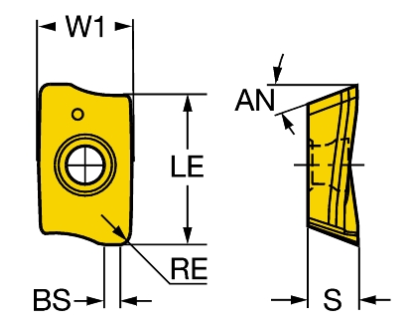
\includegraphics[width=0.5\textwidth]{insert.png}
    \caption{Insert/Workpiece Contact}
    \label{fig:insertfig}
\end{figure}

\begin{equation}
    L_e=2B_s + (a-R_e) + \frac{2R_e\pi}{4}
\end{equation}

% Table generated by Excel2LaTeX from sheet 'Sheet1'
\begin{table}[htbp]
  \centering
  \caption{Effective Cutting Edge Lengths}
    \begin{tabular}{|l|rrrr|}
    \hline
          & \multicolumn{1}{l}{Cut \#1} & \multicolumn{1}{l}{Cut \#2} & \multicolumn{1}{l}{Cut \#3 } & \multicolumn{1}{l|}{Cut \#4} \\
    \hline
    Effective Cutting Edge (in) & 0.2125 & 0.2125 & 0.2625 & 0.2625 \\
    \hline
    \end{tabular}%
  \label{tab:Le}%
\end{table}%

Then by using the cutting torques found empirically in table \ref{tab:torques} we can form a system of linear equations to solve for the force equations. Since there are only 2 unknowns we only need two equation to form the system. We can use the other two equations to confirm the number that we get from the first system.

\pagebreak
The solutions of the systems are shown in table \ref{tab:solntosys}:
% Table generated by Excel2LaTeX from sheet 'Sheet1'
\begin{table}[h!]
  \centering
  \caption{Solution to Systems}
    \begin{tabular}{|l|cc|}
    \hline
          & System w/ \#1 \& \#2 & System w/ \#3 \& \#4 \\
    \hline
    $K_1$    & 124570.98 & 124570.98 \\
    $K_2$    & 230.80 & 228.12 \\
    \hline
    \end{tabular}%
  \label{tab:solntosys}%
\end{table}%

Thus the force constants are:
\begin{empheq}[box=\fbox]{align}
    K_1&\approx124571\nonumber\\
    K_2&\approx229
\end{empheq}

\section{Conclusion}
By doing this lab we are able to better understand how the force constants are empirically found for tool/workpiece combinations. Overall this lab was effective in showing us the milling operation and how to solve for unknowns using the formulas given in the lecture notes.
\pagebreak

\appendix
\section{Matlab Code}
\lstinputlisting[style=Matlab-editor, basicstyle=\mlttfamily\scriptsize, caption={Matlab Code for Solving for Force Constants}]{MSE480_Lab1.m}
\pagebreak
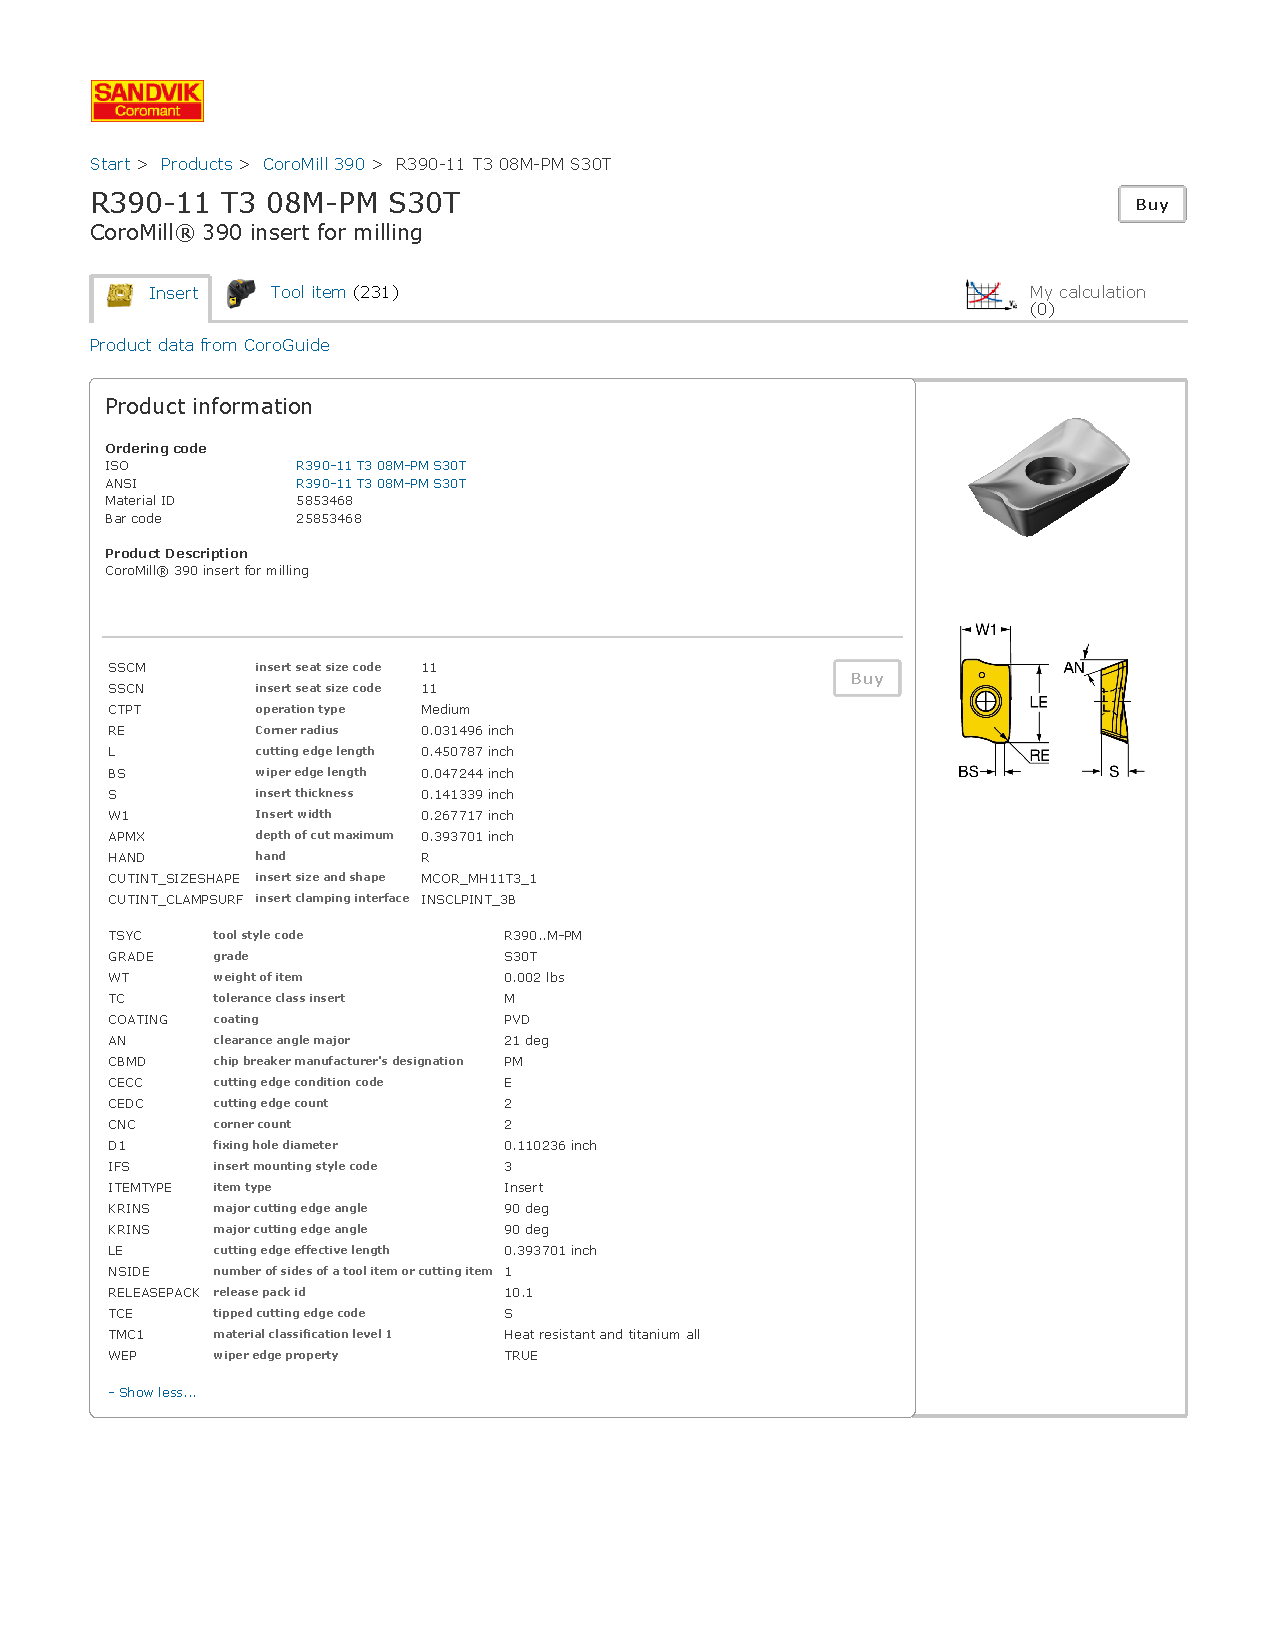
\includepdf[page=-, width=1\textwidth,pagecommand=\section{Cutting Insert Data Sheet}]{Insert_DS}
\end{document}
              
            